\chapter{Background}
\label{chapt:background}


One of the earliest citations in the neural network literature can be traced back to Rosenblatt's invention of the perceptron~\citep{rosenblatt1958perceptron} based on the work of \citet{mcculloch1943logical}.
The perceptron is equivalent to a single-layer, feed-forward, neural network, where the input vector is multiplied by a matrix, and then projected through static nonlinear activation units (e.g., a threshold function, sigmoid function, rectified linear function, or similar).\footnote{A constant bias term is usually added to the weights, to control the activation threshold of each unit.}
This static nonlinearity is intended to correspond to the abstract behaviour (i.e., average activation level) of an artificial ``neuron'', while the matrix corresponds to the synaptic weights of each neuron -- hence the term ``weight matrix''.
The output(s) of the network provide a classification of the input vector -- the interpretation of which is task-dependent.
The weight matrix is learned from example data, in a black-box manner, by applying a simple delta rule that, in effect, performs gradient descent on a loss function across the training data.

A great deal of excitement was fueled by claims that the perceptron would soon ``be able to walk, talk, see, write, reproduce itself and be conscious of its existence''~\citep{historyofperceptrons}.
But soon after, a famous book by \citet{minsky1969perceptrons} pointed out a serious limitation of this architecture: it can only classify linearly-separable patterns -- that is, it can only compute functions whose outputs distinguish its inputs based on whether the vector falls onto one side of a hyperplane or the other.
The XOR function is perhaps the simplest example of a function that \emph{cannot} be computed in such a manner.
As a brief aside, many have credited this book as bringing upon the ``AI winter'' of the 1970s: neural network architectures were soon abandoned in favour of symbol-based architectures and so-called production systems, in which general aspects of human-like intelligence are reproduced by the manipulation of abstract symbolic representations~\citep{historyofperceptrons, newell1972human}.

Fortunately, additional layers permit the computation of more complicated nonlinear functions.
That is, multi-layer feed-forward networks do not suffer the severe limitation of requiring linear-separability.
By merely stacking two perceptrons together (i.e., introducing a ``hidden layer''), the network becomes able to compute any bounded continuous function---a result known as the universal approximation theorem~\citep{hornik1989multilayer}---assuming the nonlinear activation units are bounded and continuous themselves.
This insight, together with the stacking of deeper layers to compose increasingly-complicated functions with fewer neurons, the use of ``backpropagation''~\citep{werbos1974beyond, rumelhart1986learning}---performing gradient descent across multiple layers via the chain rule---to learn all of the weight matrices, combined with increasingly-powerful GPUs to process large datasets, all coalesced to usher in the reviving era of ``deep learning''~\citep{sejnowski2018deep}.

Deep learning has undoubtedly brought about many rapid and impressive advances to the field of artificial intelligence.
Due to its black-box nature, neither domain expertise nor understanding of the network's internal function are required in order to achieve state-of-the-art performance on a large number of important problems, including: image recognition, speech recognition, natural language understanding, question answering, and language translation~\citep{lecun2015deep}.
The basic recipe is conceptually simple: obtain one of the many popular off-the-shelf toolboxes for deep learning, pick your favourite network architecture, set its hyperparameters, and then throw as much training data at the network as your GPU(s) can handle.
Deep learning excels at constructing static vector functions, that generalize to new examples, by automatically discovering the latent (i.e., hidden) low-dimensional representations that are most relevant to the task at hand.
However, the opacity of its optimization procedure comes as a double-edged sword: while it is easy to apply deep learning to many problems with minimal hand-engineering, it is unclear even to experts what effect most hyperparameter changes will have in advance on overall performance~\citep{bergstra2012random}.
For example, it has been observed that using a rectified linear~(ReLU) activiation unit for each nonlinearity can dramatically reduce the training time on a variety of benchmarks~\citep{glorot2011deep}, yet, as far as we know, this observation still does not have any theoretically-grounded framework that could assist in selecting nonlinearities or related hyperparameters for some given task.

Despite its breakthroughs, the field is well-aware that a feed-forward architecture is incapable of learning temporal relationships that span arbitrarily across the input data, which is necessary for tasks involving video, speech, and language understanding with long-range dependencies~\citep{bengio1994learning}.
Regardless of the depth of the network, a feed-forward network will always have some finite input response, which leaves a finite ``memory'' of previous inputs within the state of the network.
In other words, the functions that are computable with such a network cannot access inputs that go beyond the depth of the network.
The most general solution to overcome this problem is to introduce recurrent connections into the network, which transmit current state information back to itself, thus allowing the network to capture information about previous inputs and reuse it in the future. 
These networks are called Recurrent Neural Networks~(RNNs).

We begin with a brief theoretical discussion on the computational power of RNNs, followed by an overview of many of the most popular architectural approaches and methods to building RNNs.
This is not intended to provide a comprehensive record of all such findings, but rather to help situate this work and shine a spotlight on many of the key ingredients that motivate our eventual approach.
Reviews and references that provide more detailed accounts of these methods and its variants are included throughout.
We then describe, in detail, the three principles of the Neural Engineering Framework~\citep[NEF;][]{eliasmith2003a} while contrasting this approach with those discussed thus far.
This leads into a high-level overview of a few promising neuromorphic architectures that have been made available to us through various collaborations: SpiNNaker~\citep{furber2014spinnaker}, Braindrop~\citep{braindrop2019}, and Loihi~\citep{davies2018loihi} -- all of which support the compilation of NEF networks, and are the targets of many of our example applications.
Finally, we provide some necessary mathematical background on dynamical systems.

\section{Recurrent Neural Networks}

The Recurrent Neural Network~(RNN) is the most computationally-powerful brand of neural network that we know how to physically implement.
By using recurrent connections to persist state information through time, thus endowing the network with an internal memory, RNNs are able to compute functions outside the computational class afforded by deep feed-forward networks: \emph{dynamical systems} -- functions whose state evolves nonlinearly according to the history of its inputs.
This enables the network to exploit patterns in the input that span time along arbitrary temporal scales.

Specifically, RNNs serve as a universal approximator to any finite-dimensional, causal, discrete-time, dynamical system~\citep{schafer2006recurrent}.
That is,
\begin{equation}
\begin{aligned} \label{eq:discrete-dynamical-system}
\V{x}\left[ t + 1 \right] &= \V{f}\left(\V{x}\left[ t \right], \V{u}\left[ t \right] \right) \\
\V{y}\left[ t + 1 \right] &= \V{g}\left(\V{x}\left[ t \right] \right)
\end{aligned}
\end{equation}
where $\V{x} \in \mathbb{R}^d$ is a finite-dimensional ($d \in \mathbb{N}$) state-vector, $\V{u}$ is some input vector, and $\V{y}$ is some output vector -- all indexed at discrete units of time, $t$.
The state updates according to a nonlinear mixing of itself with the input.
The output is a static mapping (i.e., ``readout'') of the state.
The causality constraint implies that these functions do not require knowledge of future inputs (although they are free to make predictions).
% Intuitively, the input and recurrent connections correspond to $\V{f}\left(\cdot, \cdot\right)$ while the outputs correspond to $\V{g}\left(\cdot\right)$.
Crucially, an RNN with sufficiently many nonlinear units can approximate any instantiation of equation~\ref{eq:discrete-dynamical-system} arbitrarily well.

On the other hand, the human brain itself, is a highly recurrent system~\citep{dayan2001theoretical}.
Assuming its mechanisms obey the laws of physics, it must also necessarily be a dynamical system~\citep{amit1989modeling, mckenna1994brain, port1995mind}.
And unless the brain harnesses quantum physics---which is argued to be irrelevant to cognitive function~\citep{litt2006brain}---is a ``hypercomputer'' or a ``super-Turing'' computer---which is argued to require unphysical resources~\citep{broersma2018computability}---its dynamics must also be finite-dimensional.
Causality follows from assuming the brain does not violate the second law of thermodynamics~\citep{evans1996causality}.
In essense, we assume that the brain is a physical ``machine'' with finite spatiotemporal resources and limited precision.
% \footnote{The discrete-time nature of these equations is not of relevance to this discussion; as we are dealing with approximations of a physically-realizable system, a continuous-time version may be discretized with sufficiently small time-step to obtain a system in the form of equation~\ref{eq:discrete-dynamical-system}.}
From this position, it follows that the class of computations made available by RNNs is at least as large as the class of computations that can be performed by the brain.
Constraints on the physical devices leveraged by the brain (i.e.,~constraints on timing, connectivity, precision, and so forth) are likely to impose limitations that make RNNs strictly more powerful in theory.

In summary, the field of neural network theory has progressed from: the perceptron, which had the problem of not being powerful enough; to the multi-layer feed-forward network, which is a universal approximator to static functions; and finally to the RNN, which is a universal approximator to physically-implementable dynamical systems, for which we consider the brain to be an instance.
Thus, while feed-forward networks are fundamentally incapable of reproducing human intelligence, RNNs are, at least in theory, up to the task.

% Then why have RNNs not yet successfully displayed human levels of intelligence?
In practice, for tasks that involve sequential inputs, such as speech and language, RNNs are often the best choice~\citep{lecun2015deep}.
Recent instances have demonstrated impressive human-like intelligence in generating captions from images~\citep{vinyals2015show}, recognizing speech in multiple languages~\citep{amodei2016deep}, and decoding human emotions from video~\citep{ebrahimi2015recurrent}.
However, the largest RNN that we are aware of to be successfully trained is a 6.6~million neuron model of human cognition---just shy of 0.01\% the size of the human brain---using the methods of the NEF~\citep{choo2018}.
The next largest (non-NEF) RNN that we can find with published resource counts is a ``large scale'' speech recognition example from Google that consists of \numprint{6800} units in its largest instantiation~\citep[][Table~1]{sak2014long} -- on the order of \numprint{e6}--\numprint{e7} times smaller than the human brain, depending on how one counts a ``neuron'' in such a network.

Clearly, the practical and theoretical challenges lie in scaling.
As informed by the ``no free lunch theorem'' for RNNs~\citep{wiklicky1994non}, there exists no universal training algorithm that will find the correct solution to all tasks.
It is instead necessary to constrain the solution space with prior knowledge.
% Generally, the challenge is in imposing the right set of constraints that will allow one to learn the weights with some training procedure, all while remaining implementable within some available resource and power budget. % order of \numprint{e11}~neurons and \numprint{e14}~weights.
This has motivated the invention of many different types of RNNs and training methods, a selection of which are described in the following sections.
For more information we point the reader to a review by \citet{salehinejad2017recent}.

\subsection{Backpropagation Through Time}

The traditional approach to build an RNN is to take a single-layer feed-forward network, and recurrently connect the output of each neuron to all other neurons in the same layer with a square weight matrix.
To simulate the network, the weighted activations propagated by the recurrent feedback loop are delayed by a single time-step, and added to the weighted inputs on the next step.
To train the network, we apply backpropagation through time~\citep[BPTT;][]{werbos1990backpropagation}.
Intuitively, the idea is to ``unroll'' the network in time, and treat it as an infinitely-deep feed-forward network where the input at the $i^\text{th}$ time-step, together with the output from the $(i-1)^\text{th}$ layer, are supplied to the $i^\text{th}$ layer.
This may optionally be stacked to form multiple layers, akin to a multi-layer feed-forward network where each layer is locally recurrent~\citep{pascanu2013construct}.

This approach also extends to more biologically-plausible realizations of the RNN, in which the continuous (i.e.,~real-valued) neural activations are replaced by spiking neurons that emit binary-valued events over time, and weight matrices are replaced by synaptic filters that appropriately weight and exponentially decay incoming spikes over time.
These networks are named Spiking Neural Networks~(SNNs), and are the subject matter of later sections.
The issue in this context is that spikes (i.e.,~Dirac impulses) are non-differentiable with respect to time.
But recently, many research groups have independently demonstrated that SNNs can also be trained with backpropagation by softening the gradient in a variety of creative ways~\citep{hunsberger2015spiking, hunsberger2016training, marblestone2016toward, neftci2017neuromorphic, bellec2018long, hunsberger2018, huh2018gradient, severa2018whetstone, rasmussen2018nengodl, neftci2019surrogate}.
Likewise, it was recently shown by \citet{chen2018neural} that both RNNs and backpropagation can be extended to continuous-time (i.e.,~taking the limit of infinitesimally small time-steps), consistent with the the NEF and Principle~3~(see section~\ref{sec:principle3}).
 
While these approaches are theoretically sound, BPTT encounters many problems in practice~\citep{bengio1994learning}.
Chief among these are the so-called ``vanishing and exploding gradient problems'', in which gradients shrink or grow unboundedly as they are propagated back in time.
These problems are intimately related to the ``credit-assignment problem'', in which a learner witnesses a combinatorial explosion of points in time to assign credit to for the current error; in the case of storing a single bit of information over time, this causes the gradient to be inherently unstable~\citep{bengio1994credit}.
Thus, a standard RNN trained by BPTT will often fail to learn tasks that require a longer term memory -- a serious problem for the use-cases that RNNs promise to address.
Solutions proposed by \citet{pascanu2013difficulty} that involve clipping and constraining the gradients alleviate these problems to some extent, but the issue still rears its head in toy tasks that are of relevance to theoretical neuroscience~\citep{depasquale2018full}.
Alternatives to BPTT include extended Kalman filter-based learning, second-order Hessian-based optimization methods, Hessian-free optimization, and evolutionary algorithms~\citep{salehinejad2017recent} -- but none have been found to be as consistently useful in practice as backpropagation.
To face the problem of learning across longer time-scales, architectural constraints are often imposed on the RNN, such as those in the following section.

\subsection{Structured Approaches}

The Long Short-Term Memory~\citep[LSTM;][]{hochreiter1997long} network addresses the problem of storing information across long intervals of time, by incorporating an explicit memory unit into the network.
Rather than a static nonlinearity, the basic computational element is an LSTM ``cell'': a group of five nonlinearities and three multiplicative gates, dynamically coupled to one another in a specific manner, such that its default behaviour is to ``store'' its input, by propagating an internal state variable back to itself on the next time-step (i.e.,~using an internal feedback connection).
Multiplicative gating controls whether the input should be integrated, whether the memory is to decay with some leakage, and whether to output the contents of the memory~\citep{gers1999learning}.
Importantly, all of these mechanisms are differentiable, and so BPTT can be applied to automatically learn all of the gating parameters.
Thus, the LSTM can be viewed as a particular way of configuring and initializing an RNN in a manner that assists BPTT, by biasing it towards latching onto values and persisting them for long, yet controlled, periods of time.

The LSTM reduces the vanishing and exploding gradient problems, described in \citet{bengio1994learning}, by restructuring the gradient that is involved when integrating over time.
The standard practice is to create layers of LSTM cells, and then stack several of these layers on top of one another, using weight matrices to fully connect each layer to the next~\citep{graves2013speech}.
This enhances the temporal complexity of the network's dynamics through a composition of time-scales, analogous to the manner in which deep feed-forward networks provide richer internal representations via composition of spatial scales.
Recently, this has found success in sequence learning, machine translation, and speech~\citep{graves2013speech, sutskever2014sequence, cho2014learning, bahdanau2014neural}, leading to a widespread adoption of LSTM networks as the RNN of choice~\citep{lecun2015deep}.

A spiking analog to LSTMs have also been proposed by \citet{bellec2018long}, in which adaptive neurons take on the functional role of LSTM cells.
The intuition behind why this works is that the adaptive state of the neuron is functionally similar to that of a controlled leaky integrator.
When BPTT is applied to such an SNN, it has been shown to approach the performance of a non-spiking LSTM network.
The structure of LSTM cells have also been compared to that of cortical microcircuits in biology, providing a post hoc explanation for the utility of LSTMs~\citep{costa2017cortical}.

This success has prompted many variants of LSTMs, including the bidirectional LSTM~\citep{graves2005framewise}, hierarchical S-LSTM~\citep{zhu2015long}, grid LSTM~\citep{kalchbrenner2015grid}, phased LSTM~\citep{neil2016phased}, and others~\citep{salehinejad2017recent}.
At the same time, this has inspired several related architectures that augment an RNN with differentiable memory cells to facilitate long-range temporal interactions, including the gated recurrent unit~\citep[GRU;][]{cho2014properties, chung2014empirical}, neural Turing machine~\citep{graves2014neural}, memory network~\citep{weston2014memory}, and orthogonal GRU~\citep{jing2018gated}.
In section~\TODO{reference LSTM-DelayCell comparison section}, we propose another kind of memory cell based on our work, and compare their performance in terms of memory capacity to LSTMs.
Results on a chaotic time-series prediction benchmark suggest that LSTMs, when interleaved with our novel memory cell, and trained via BPTT, become capable of learning systems described by nonlinear delay-differential equations.

\subsection{Randomized Approaches}

Reservoir Computing~(RC) is a strategy for training RNNs, that relaxes the optimization problem by keeping the recurrent weights fixed.
That is, only the static ``readout'' weights to a linear output layer are modified, while the recurrent weights are left untrained, thus sidestepping the issues in BPTT.
This is referred to as an Echo State Network~\citep[ESN;][]{jaeger2001echo}, or Liquid State Machine~\citep[LSM;][]{maass2002real}, depending on whether the neural nonlinearities are static or spiking models, respectively.
The intuition is that randomized feedback, when initialized in an appropriate manner, causes traces of the input to dynamically reverberate, or ``echo'', throughout the state of the network; a common metaphor is depicted by throwing rocks into a pool of water and observing the ripples interact through time.\footnote{To demonstrate the relevance of this metaphor, \citet{fernando2003pattern} went so far as to actually implement an LSM using a bucket of water.}
These traces can then be decoded to reconstruct the output signal in a manner that approximates a nonlinear transfer function of the input signal.
Details are provided in section~\ref{sec:relationships} after introducing the NEF.

There are two great insights driving the adoption of RC: (1) randomized feedback provides an overcomplete basis of nonlinear time-varying signals that can be linearly combined to approximate some target signal, and (2) by leaving the recurrent weights fixed, the optimization procedure is greatly simplified; training the readout weights amounts to a least-squares problem.
However, the benefits of RC do not come without limitations involving memory capacity. \TODO{Cite some key results.}
In particular, section~\ref{sec:delay-rc} compares the performance of RC to the NEF on a continuous-time memory benchmark, thus highlighting severe scaling issues with RC.

\subsection{Engineered Approaches}

A unique set of approaches to training RNNs is rooted in the application of engineering and control-theoretic methods to modelling neurobiological systems~\citep{eliasmith1999developing}.
We call these top-down methods ``engineered approaches''.
These methods all assume that some model of the system's desired dynamics (i.e.,~$\V{x}$ in equation~\ref{eq:discrete-dynamical-system}) are known apriori.
That is, rather than suppose our only knowledge is raw input-output data, many real-world scenarios provide opportunities to model the dynamical system that actually generated the data.
In practice, this might be some physical model of the dynamical system under consideration, an approximate model that has been identified~\citep{nelles2013nonlinear}, or even some partial observation of the dynamical state.
Often, the dynamical system is simply a description of a particular computation that we know to be useful, such as a controller for a robotic arm, or the examples provided in section~\ref{sec:dynamics-language}.

Instances of this approach include the Neural Engineering Framework~\citep[NEF;][]{eliasmith2003a, duggins2017incorporating}, first-order reduced and controlled error~\citep[FORCE;][]{sussillo2009generating, depasquale2018full} and its spiking relatives~\citep{nicola2016supervised, thalmeier2016learning}, balanced spiking networks~\citep{boerlin2011spike, boerlin2013predictive, schwemmer2015constructing, alemi2018learning}, and closely-related methods~\citep{jaeger2014controlling, gilra2017predicting}.
Reviews of many of these methods are given by \citet{deneve2016efficient} and \citet{abbott2016building}, and we discuss some of the critical points below.
In all cases, these methods provide a procedure for taking a description of some desired dynamical state-vector, and then training a recurrent network of spiking or non-spiking neurons, with varying constraints on the target models' level of biological detail, to represent that state.

It is important to note that, although all of these approaches are engineered from a top-down modelling perspective, one can still apply BPTT (or any other optimization method) to fine-tune the resulting RNN end-to-end from example input-output pairs -- a hybrid approach that is embraced by the NEF and its software stack~\citep{rasmussen2018nengodl}.
The point is that prior knowledge of the task can help place appropriate constraints on the initial configuration of the RNN to assist BPTT, and provide transparency into the relationships between network parameters, configuration, and function.
This transparency enables theoretical insights into neural computation, and, as we will show, practical advances on RNN benchmarks that would otherwise be quite difficult to obtain with a pure black-box approach.

In section~\ref{sec:nef} we provide a detailed account of the NEF, and in section~\ref{sec:relationships} we draw architectural comparisons to both RC and FORCE.
Its extension, full-FORCE~\citep{depasquale2018full}, can be viewed an an instance of the NEF with full-rank weight matrices~\citep{tripp2006neural}, where training is performed online rather than offline, and randomized feedback is thrown in to serve the same purposes as in RC.
The methods of \citet{thalmeier2016learning} provide a means of realizing FORCE and full-FORCE networks in biologically plausible spiking networks using a precise spike-time coding mechanism, similar to ~\citet{boerlin2013predictive}, supported by nonlinearities in the synapses.
On the other hand, \citet{jaeger2014controlling} can be viewed as an extension of RC that is essentially an offline variant of FORCE, or a non-spiking NEF network~\citep{aubin2017}.

Balanced spiking networks also share many commonalities with the NEF, primarily a procedure for mapping a dynamical state vector onto a population of spiking neurons, via a low-rank weight matrix that accounts for the dynamics of the neurons and synapses.
The main benefit of the balanced network approach is that precision scales as $\bigoh{n}$, compared to $\bigoh{\sqrt{n}}$ for the NEF, where $n$ is the number of neurons, by carefully coordinating the variance in spike-timing~\citep[][Figure~11]{boahen2017neuromorph}.
However, this scheme only applies to linear dynamical systems, relies on assumptions of near-instantaneous communication between all neurons, and requires linear neurons with minimal leakage and no refractory period~\citep{boerlin2013predictive}.
\citet{schwemmer2015constructing} has extended these methods to support more biologically plausible models, but the scaling benefits do not appear to persist beyond $100$--$400$ neurons~[personal communication].
In general, it is unclear how far these assumptions can be relaxed before scaling regresses to $\bigoh{\sqrt{n}}$, which is of relevance when considering our targets of modelling biological systems and mapping onto neuromorphic hardware -- both of these targets regularly violate the above assumptions.

Given the subtle distinctions between these similar sets of approaches,
section~\ref{sec:nef-suitability} rigorously analyzes the suitability of the NEF for universal spike-based computation on neuromorphic hardware.
The NEF is mathematically correct under fairly weak assumptions, which leads to it being robust and extensible.
These key factors contribute to the NEF being our toolkit of choice when it comes to training RNNs for the purposes of deployment on the neuromorphic hardware summarized in section~\ref{sec:neuromorphic}.

\TODO{Mention all of the methods for converting ANNs to SNNs at some point (apart from backprop on SNNs). Including \citep{rueckauer2017conversion} and related background and sigma-delta and \citep{yousefzadehconversion2019} and etc.}

\section{Neural Engineering Framework}
\label{sec:nef}

\TODO{Quickly compare and contextualize against the above}

\citep{dynamicspatent}
\citep{sussillo2013opening}

\citep{hunsberger2015spiking, hunsberger2016training, hunsberger2018, rasmussen2018nengodl}

One of the central challenges in computational neuroscience is understanding how dynamic stimuli can be processed by neural mechanisms to drive behavior.
Recurrent connections, cellular responses, and synaptic responses are ubiquitous sources of dynamics throughout the mammalian brain that must work in concert to support dynamic information processing~\citep{kandel2000principles}.
How these low-level mechanisms interact in order to encode information about the history of a stimulus, across time, is the subject of considerable study.
One approach to better understanding these mechanisms is to construct models that capture central features of neural dynamics, while implementing higher-level information processing.


%The ways in which these low-level mechanisms might interact, in order to usefully encode information about a stimulus \emph{across time}, are generally unclear in the context of high-level cognition~\citep{?}.

% Biology has appeared to solve this problem by imposing structure in the brain, with neuroanatomical constraints that differ considerably by brain area~\citep[][pp.~207--227]{kandel2000principles}.
% We interpret this pragmatically as a need to: (1) incorporate prior knowledge of a desired function into the structure of a network, and (2) constrain a network's topology using known properties of the underlying dynamical mechanisms.

The Neural Engineering Framework~\citep[NEF;][]{eliasmith1999developing, eliasmith2003a} proposes a method to model such dynamical systems in networks of spiking neurons~\citep[see][for reviews of other methods]{abbott2016building, deneve2016efficient}.
The NEF has been used to construct a wide variety of neural models, including a 2.3 million neuron functioning model of the human brain, named ``Spaun'', capable of performing perceptual, motor, and cognitive tasks~\citep{eliasmith2012}.
This model incorporates many kinds of observed neural dynamics, including oscillations, sustained activity, and point attractor dynamics.
The flexibility of the NEF has lead to it being deployed on mixed-analog-digital neuromorphic chips~\citep{choudhary2012silicon, corradi2014, voelker2017iscas, voelker2017neuromorphic} and digital architectures~\citep{bekolay2013, wang2014compact, mundy2015efficient, berzish2016}.
Consequently, the NEF provides a practical method for programming neuromorphics, thus helping the field realize its promise of a low-energy computing platform that emulates core principles of the nervous system~\citep{boahen2017neuromorph}.

However, the NEF typically assumes an exponential model of the post-synaptic current~(PSC) evoked by an action potential, which has a biologically implausible, instantaneous rise-time.
This model is also known as a first-order lowpass filter.
In contrast, the synapse models used in mixed-analog-digital neuromorphic chips are nonideal, featuring higher-order dynamics due to parasitic capacitances~\citep{voelker2017iscas}.
Similarly, the synapse models commonly used in biological models incorporate distinct rise- and fall-times due to separate time scales of transmitter binding and unbinding, as well as axonal transmission delays due to the finite-velocity propagation of action potentials~\citep{roth2009modeling}.
To widen the scope of the NEF, we characterize the network-level effects of these higher-order synapse models, and harness them to implement certain classes of dynamical systems with improved accuracy.

A particularly important dynamical system that has not been implemented using the NEF is the pure continuous-time delay line.
This system must represent a rolling window of input history.
We provide a novel derivation of an optimal low-dimensional linear approximation to a continuous-time delay, and prove that the resulting \emph{delay network} nonlinearly encodes its input across the delay interval.
This network uses a scale-invariant representation, with a level of accuracy that depends on the input frequency, chosen dimensionality (i.e.,~the order of the approximation), and particular synapse model.
Low-dimensional representations (e.g.,~$\le 27$) of low-frequency signals (e.g.,~$\le 50$\,Hz) are pervasive in biological systems~\citep{cunningham2014dimensionality, waernberg2017low, pulvermuller1997high, singer1999neuronal}.
To our knowledge, this work is the first to demonstrate that such a temporal code may be accurately implemented using a spiking dynamical network.

Reservoir Computing approaches, such as Liquid State Machines~\citep{maass2002real} and Echo State Networks~\citep{jaeger2001echo}, may be used to approximate a delay line.
However, since these networks use randomly chosen feedback weights, it is likely that they do not {\it efficiently} produce the dynamics of a pure delay.
Rather, these networks represent a random variety of nonlinear memory traces~\citep{lukovsevicius2012reservoir}.
Discrete approaches to short-term memory, such as those taken by \citet{white2004short} and \citet{ganguli2008memory}, while optimal in an information-theoretic sense, rely fundamentally on single time-step delays between rate-based neurons.
In contrast, the method that we propose here works independently of the simulation time-step, and is optimal assuming the population of spiking neurons---coupled with some model of the synapse---accurately represents a low-dimensional, low-frequency, vector space.
Furthermore, our framework is extended to account for arbitrary linear synapses, which improves our understanding of the relationship between synapse models and network-level computation.
A detailed comparison of our method to Reservoir Computing remains the subject of future work.

A distinguishing feature of this work is that we begin the problem with a mathematical description of the ideal dynamics for the delay line, and then proceed by mapping this description onto a spiking neural network (using the NEF and its extensions).
This is in contrast to methods that use online learning or backpropagation through time with rate-based neurons~\citep{de1992gamma, sussillo2009generating} or spiking neurons~\citep{nicola2016supervised, huh2017gradient, gilra2017predicting, alemi2017learning}.
That is, we do not require any sophisticated training regimes involving online learning or backpropagation; our delay network is trained offline using convex optimization~(i.e.,~regularized least-squares), which yields a more complete understanding of its employed representation and dynamics.

The Neural Engineering Framework~\citep[NEF;][]{eliasmith1999developing, eliasmith2003a} consists of three mathematical principles used to describe neural computation.
The NEF is most commonly applied to building dynamic (i.e.,~recurrent) spiking neural networks, but also applies to non-spiking and feed-forward networks.
Its primary strength lies in providing a well-understood and efficient means of engineering spiking neural models, and programming neuromorphic hardware, to perform mathematically described computations~\citep{eliasmith2013build, boahen2017neuromorph}.
In this section, we provide an overview of these methods applied to training both feed-forward and recurrent connection weights, in order to implement linear dynamical systems -- although these methods extend to nonlinear dynamical systems as well~\citep{voelker2017iscas, voelker2017neuromorphic}.
We present this framework in a manner that is consistent with the Nengo~2.4.0 simulator~\citep{bekolay2013}, which implements the NEF among other approaches.

\subsection{Principle 1 -- Representaiton}
\label{sec:principle1}

Let $\V{x}(t) \in \mathbb{R}^q$ denote a $q$-dimensional time-varying signal, that is to be represented by a population of $n$ spiking neurons.
To describe this representation, we define a nonlinear \emph{encoding} and a linear \emph{decoding} that together determine how neural activity relates to the represented vector.

First, we choose encoders $E = \transpose{\left[ \V{e}_1\text{,}\, \ldots\text{,}\, \V{e}_n \right]} \in \mathbb{R}^{n \times q}$, gains $\alpha_i > 0$, and biases $\beta_i$, $i = 1 \ldots n$, as parameters for the encoding, which map $\V{x}(t)$ to neural activities.
These parameters are fit from neuroanatomical data (e.g.,~tuning curves, preferred directions, firing rates, sparsity, etc.; see \citet{voelker2016a} for a recent example), or randomly sampled from distributions constrained by the domain of $\V{x}(t)$ and the dynamic range of the neuron models.
% Most often, we select distributions from which to sample these parameters, incorporating known constraints on the system under consideration.
In either case, the encoding is defined by:
\begin{equation} \label{eq:encoding}
a_i^\V{x}(t) = G_i \left[ \alpha_i \left\langle \V{e}_i, \V{x}(t) \right\rangle + \beta_i \right] \text{,} \quad i = 1 \ldots n \text{,}
\end{equation}
where $a_i^\V{x}(t)$ is the neural activity generated by the $i^{\text{th}}$ neuron encoding the vector $\V{x}(t)$ at time $t$, $\left\langle \cdot , \cdot \right\rangle$ denotes a dot-product, and $G_i[\cdot]$ is the nonlinear dynamical system for a single neuron (e.g.,~a leaky integrate-and-fire~(LIF) neuron, a conductance-based neuron, etc.).
Then $a_i^\V{x}(t) = \sum_m \delta \left(t - t_{i\text{,}m} \right)$, where $\delta(\cdot)$ is the Dirac delta, and $\left\{ t_{i\text{,}m} \right\}$ is the sequence of spike-times generated by equation~\ref{eq:encoding}. % via $G_i \left[ \cdot \right]$.

Having defined an encoding, we introduce a postsynaptic filter $h(t)$, which acts as the \emph{synapse model} by capturing the dynamics of a receiving neuron's synapse.
In particular, this filter models the postsynaptic current (PSC) triggered by action potentials arriving at the synaptic cleft.
For now, we fix $h(t) = \frac{1}{\tau} e^{-\frac{t}{\tau}}$ to be an exponentially decaying PSC with time-constant $\tau$, which is equivalent (in the Laplace domain) to the canonical first-order lowpass filter (also known as a ``leaky integrator'').
This is the conventional choice of synapse in the NEF, since it strikes a convenient balance between mathematical simplicity and biological plausibility~\citep{eliasmith2003a}.
In section~\ref{sec:extensions}, we return to this point by considering more general synapse models that are capable of capturing a much broader variety of PSCs.

We can now characterize the decoding of the neural response, which determines the information extracted from the neural activities encoding $\V{x}(t)$.
Let $D = \transpose{\left[ \V{d}_1\text{,}\, \ldots\text{,}\, \V{d}_n \right]} \in \mathbb{R}^{n \times q}$ be the decoding matrix that decodes $\V{x}(t)$ from the population's activities $\left( a_i^\V{x}(t) \right)$ at time $t$.
This linear decoding is described by:
\begin{equation} \label{eq:rep-decode}
\left(\V{x} \ast h \right)(t) \approx \sum_{i=1}^n (a_i^\V{x} \ast h)(t) \V{d}_i \text{,}
\end{equation}
where $\ast$ is the convolution operator that is used to apply the synaptic filter.
Equation~\ref{eq:rep-decode} takes a linear combination of the filtered activities, in order to recover a filtered version of the encoded signal.\footnote{It is more accurate to apply the filter to both sides, since in general the (time-invariant) decoders alone cannot compensate for the filter applied to the activities (this instead becomes the role of Principle~3).}
To complete the characterization of neural representation, we solve for the optimal linear decoders $D$.
This optimization is identical for Principles~1 and 2, as discussed below.

\TODO{Discuss some scaling}

Anectodally (e.g., personal conversation with Sophie Den\`eve, experience with Nengo, and averages in Spaun), we say 50-100 neurons per dimension achieves tolerable levels of noise.
For a fixed amount of noise in a represention implemented by an ensemble of $n$ neurons, the current best-known lower-bound predicts the dimensionality $d$ scales as $\Omega \left( n^{\frac{2}{3}} \right)$ for $n$ neurons~citep[][p.~60]{jgosmann2018}.
Although we don't know the upper-bound, we conjecture that it is $\bigoh{n}$.
That is, the dimensionality should not be able to scale faster than the neuron count.
If it could, then each neuron would represent $\omega(1)$ dimensions, which seems physically implausible given access to only $\bigoh{1}$ state variables.
This limitation could be broken by dendritic computation, for instance if each neuron had access to $\bigoh{n}$ variables distributed along the dendritic tree.

\subsection{Principle 2 -- Transformation}
\label{sec:principle2}

The second principle of the NEF addresses the issue of computing transformations of the represented signal.
The encoding remains defined by equation~\ref{eq:encoding}.
However, we now decode some desired function of $\V{x}(t)$, $\V{f} : \mathbb{R}^q \rightarrow \mathbb{R}^q$,\footnote{
We may also consider transformations where the range has a different dimension, but the described framework will suffice for our purposes.}
by applying an alternate matrix of decoders $D^\V{f} = \transpose{\left[ \V{d}^\V{f}_1\text{,}\, \ldots\text{,}\, \V{d}^\V{f}_n \right]} \in \mathbb{R}^{n \times q}$ to the same activities:
\begin{equation} \label{eq:trans-decode}
\left( \V{f}(\V{x}) \ast h \right)(t) \approx \sum_{i=1}^n (a_i^\V{x} \ast h)(t) \V{d}^\V{f}_i \text{.}
\end{equation}
For both Principles~1 and~2, we optimize for $D^\V{f}$ over the domain of the signal, $S = \{\V{x}(t) : t \ge 0\}$, which is typically the unit $q$-ball $\{ \V{v} \in \mathbb{R}^q : \|\V{v}\|_2 \le 1\}$ or the unit $q$-cube $[-1\text{,}\, 1]^q$.
To determine these decoders, we first let $r_i(\V{v})$ be the limiting average firing rate of the $i^{\text{th}}$ neuron under the constant input $\V{v} \in S$:
\begin{equation} \label{eq:rates}
r_i(\V{v}) = \lim_{t \rightarrow \infty} \frac{1}{t} \int_{0}^t a_i^\V{v}(t') \, dt' \text{.}
\end{equation}
For non-adaptive neuron models, equation~\ref{eq:rates} reduces to encoding $\V{v}$ using a rate model.
For adaptive neuron models, other definitions for $r_i(\V{v})$ may be considered, but we limit our discussion here to the (non-adaptive) spiking LIF model.
To account for the variance introduced by neural spiking, and other sources of uncertainty, we introduce a white noise term $\eta \sim \mathcal{N}(0, \sigma^2)$.
The optimality criteria for $D^\V{f}$ is therefore:
\begin{equation} \label{eq:decoder_solution}
D^\V{f} = \argmin_{D \in \mathbb{R}^{n \times q}} \int_{S} \left\| \V{f}(\V{v}) - \sum_{i=1}^n (r_i(\V{v}) + \eta) \V{d}_i \right\|^2 \, d^q\V{v} \text{.}
\end{equation}
Note that this optimization only depends on $r_i(\V{v})$ for $\V{v} \in S$, as opposed to depending on the signal $\V{x}(t)$.
In other words, the optimization is determined strictly by the distribution of the signal, and not according to its particular dynamics.
Furthermore, this is a convex optimization problem, which may be solved by uniformly sampling $S$~\citep{voelker2017} and applying a standard regularized least-squares solver to the sampled data~\citep{bekolay2013}.
Monte Carlo sampling introduces $\bigoh{ \frac{1}{\sqrt{m}} }$ error into the integral from equation~\ref{eq:decoder_solution}, where $m$ is the number of samples, but this can be improved to $\widetilde{\mathcal{O}} \left( \frac{1}{m} \right)$---effectively squaring $m$---by the use of quasi-Monte Carlo methods~\citep{fang1994, voelker2016b}.
Nengo also supports alternative decoder solvers that optimize variations of equation~\ref{eq:decoder_solution}~\citep[e.g.,][]{voelker2016a, abrams2017}, but we do not use them here.
%This provides the decoders needed by equations~\ref{eq:repn_decode} and \ref{eq:trans-decode} to represent the vector or compute transformations, respectively.

% this synapse is only for continuous case:
%\begin{equation}
%h_i(t) = \frac{1}{\tau_i} e^{-\frac{t}{\tau_i}}
%\end{equation}

The accuracy of this approach relies on $r_i(\V{v})$ being a suitable proxy for $a_i^\V{x}(t)$ whenever $\V{x}(t) = \V{v}$.
This zeroth-order approximation clearly holds in the steady-state for constant $\V{x}(t)$, and turns out to be ideal in practice for low-frequency $\V{x}(t)$~\citep[][appendix~F.1]{eliasmith2003a}, and likewise for $h(t)$ that filter out high frequencies (i.e.,~when the synaptic time-constant $\tau$ is large).
% Reminder: there's a result in my comp-II report that the expected spike train is the same as the rate model when the prior for the spike interval is uniform -- this prior becomes invalid for high frequency \V{x}(t) that cross over the neuron threshold
% We also remark that one may use singular value decomposition~(SVD) to characterize the class of functions that can be accurately approximated by the chosen neural basis functions~\citep[][pp.~185--217]{eliasmith2003a}.

Equations~\ref{eq:encoding} and \ref{eq:trans-decode} may then be used to derive a connection weight matrix between layers to implicitly compute the desired function $\V{f}(\V{x})$ within the \emph{latent} vector space $\mathbb{R}^q$.
Specifically, the weight matrix $W = [\omega_{ij}] \in \mathbb{R}^{n \times n}$, which maps activities from the $j^{\text{th}}$ presynaptic neuron to the $i^{\text{th}}$ postsynaptic neuron (disregarding the gain, bias, and synapse), is given by:
\begin{equation} \label{eq:factored-weights}
\omega_{ij} = \left\langle \V{e}_i, \V{d}^\V{f}_j \right\rangle \text{.} % = \left( \transpose{E\left( D^\V{f} \right)} \right)_{ij}
\end{equation}
%where $E$ are the encoders of the postsynaptic population from equation~\ref{eq:encoding}, and $D$ are the decoders of the presynaptic population solved by equation~\ref{eq:decoder_solution}.
Consequently, the matrices $E$ and $D^\V{f}$ are a low-rank factorization of $W$.
In other words, the process of decoding (equation~\ref{eq:trans-decode}) and then encoding (equation~\ref{eq:encoding}) is equivalent to taking the dot-product of the full-rank weight matrix $W$ with the neural activities.
% Intuitively, structure is imposed by the choice of representing $\V{x}(t)$, which in turn becomes latent within the weight matrix.

This factorization has important consequences for the computational efficiency of neural simulations.
The crucial difference between the factorized and non-factorized forms is that it takes $\bigoh{q n}$ operations per simulation time-step to implement this dot-product in the factored form of equation~\ref{eq:factored-weights}, as opposed to $\bigoh{ n^2 }$ operations for a full-rank weight matrix.
Since $q$ is typically held constant, this yields a factor $\bigoh{ n }$ improvement in simulation time.
Similarly, this factorizations yields an $\bigoh{ n }$ reduction in memory, which significantly improves the scaling of neuromorphics~\citep{mundy2015efficient}.
% including those in RC.
In essence, this factorization provides a way to describe the network's latent state-vector $\V{x}(t)$.
This, in turn, permits us to perform useful computations by transforming the state-vector with $\bigoh{ \frac{1}{\sqrt{n}} }$ error in the presence of spike-noise~\citep[][p.~47]{eliasmith2003a}.

\subsection{Principle 3 -- Dynamics}
\label{sec:principle3}

\begin{figure}
  \centering
  \resizebox{\columnwidth}{!} {
	\begin{tikzpicture}[auto, node distance=2cm,>=latex']
	  \node [input, name=input] {};
	  \node [coordinate, name=fanin, right of=input] {};
	  \node [block, right of=fanin, node distance=1.5cm] (B) {$B$};
	  \node [sum, right of=B, node distance=2cm] (sum) {$+$};
	  \node [block, right of=sum, node distance=2cm] (integ) {$\int$};
	  \node [block, right of=integ, node distance=3.5cm] (C) {$C$};
	  \node [sum, right of=C, node distance=2cm] (sumout) {$+$};
	  \node [output, right of=sumout] (output) {};
	
	  \node [block, below of=integ] (A) {$A$};
	  \node [block, above of=integ] (D) {$D$};
	
	  \draw [-] (input) -- node {$\V{u}$} (fanin);
	  \draw [->] (fanin) -- node {} (B);
	  \draw [->] (fanin) |- (D);
	  \draw [->] (D) -| node {} (sumout);
	  \draw [->] (B) -- node {} (sum);
	  \draw [->] (sum) -- node {} (integ);
	  \draw [->] (integ) -- node [name=fanout] {$\V{x}$} (C);
	  \draw [->] (fanout) |- (A);
	  \draw [->] (A) -| node {} (sum);
	  \draw [->] (C) -- node {} (sumout);
	  \draw [->] (sumout) -- node {$\V{y}$} (output);
	\end{tikzpicture}  
  }
  \caption{ \label{fig:lti-system}
    Block diagram for a LTI system.
    The integrator is driven by the signal $\dot{\V{x}}(t)$.
  }
\end{figure}

Principle~3 is a method of harnessing the dynamics of the synapse model for network-level information processing.
We begin by focusing our discussion of NEF dynamics on the neural implementation of continuous, linear time-invariant~(LTI) systems:
\begin{equation} \label{eq:lti}
\begin{split}
\dot{\V{x}}(t) &= A\V{x}(t) + B\V{u}(t) \text{,} \\
\V{y}(t) &= C\V{x}(t) + D\V{u}(t) \text{,}
\end{split}
\end{equation}
where the time-varying signal $\V{x}(t)$ represents the system state, $\dot{\V{x}}(t)$ its time-derivative, $\V{y}(t)$ the output, $\V{u}(t)$ the input, and the time-invariant matrices $(A\text{,}\, B\text{,}\, C\text{,}\, D)$ fully describe the system~\citep{brogan1982modern}.
This form of a LTI system is commonly referred to as the \emph{state-space model}, but there are many other equivalent forms, which we refer to later.

For LTI systems, the \emph{dynamical primitive}---that is, the source of the dynamics---is the integrator (see Figure~\ref{fig:lti-system}).
However, the dynamical primitive at our disposal is the \emph{leaky} integrator, given by the canonical first-order lowpass filter modeling the synapse:
\begin{align} \label{eq:lowpass}
h(t) = \frac{1}{\tau} e^{-\frac{t}{\tau}} = \mathcal{L}^{-1}\left\{ \frac{1}{\tau s + 1} \right\} \text{,}
\end{align}
where $\mathcal{L}^{-1}\{ \cdot \}$ denotes the inverse Laplace transform.\footnote{
For comparison, the Laplace transform of the integrator is $\mathcal{L}\left\{ 1 \right\} = \frac{1}{s}$.}
To be more precise, our approach is to represent the state-vector $\V{x}(t)$ in a population of spiking neurons (Principle~1;~equation~\ref{eq:encoding}), such that this vector is obtained by filtering some linearly decoded spike-trains with a leaky integrator (Principle~2;~equation~\ref{eq:trans-decode}).
Thus, the goal of Principle~3 is to determine the transformations required to implement equation~\ref{eq:lti}, given that $\V{x}(t)$ is obtained by some convolution with a leaky integrator, rather than the perfect integrator depicted in Figure~\ref{fig:lti-system}.

Principle~3 states that in order to implement equation~\ref{eq:lti} in a population of neurons that represents $\V{x}(t)$, we must compensate for the effect of ``replacing'' the integrator with a leaky integrator (compare Figures~\ref{fig:lti-system} and~\ref{fig:lti-system-mapped}), that is, by driving the synapse with $\tau \dot{\V{x}}(t) + \V{x}(t)$ instead of only $\dot{\V{x}}(t)$.
This compensation is achieved as follows: implement the recurrent transformation $(\tau A + I)\V{x}(t)$, and the input transformation $\tau B \V{u}(t)$, but use the same output transformation $C\V{x}(t)$, and the same passthrough transformation $D\V{u}(t)$~\citep[][pp.~221--225]{eliasmith2003a}.
%Because Principles~1 and~2 tell us how to represent states (i.e.,~$\V{x}(t)$) and transformations of these states (e.g.,~$(\tau A + I)\V{x}(t)$) we can use these principles to compute the necessary signals.
Specifically, this may be implemented in a spiking dynamical network by representing $\V{x}(t)$ via Principle~1 and then using Principle~2 to decode the needed transformations.
The resulting model is summarized in Figure~\ref{fig:lti-system-mapped}.

\begin{figure}
  \centering
  \resizebox{\columnwidth}{!} {
	\begin{tikzpicture}[auto, node distance=2cm,>=latex']
	  \node [input, name=input] {};
	  \node [coordinate, name=fanin, right of=input] {};
	  \node [block, right of=fanin, node distance=1.5cm] (B) {$\tau B$};
	  \node [sum, right of=B, node distance=2cm] (sum) {$+$};
	  \node [block, right of=sum, node distance=2cm] (integ) {$\frac{1}{\tau s + 1}$};
	  \node [block, right of=integ, node distance=3.5cm] (C) {$C$};
	  \node [sum, right of=C, node distance=2cm] (sumout) {$+$};
	  \node [output, right of=sumout] (output) {};
	
	  \node [block, below of=integ] (A) {$\tau A + I$};
	  \node [block, above of=integ] (D) {$D$};
	
	  \draw [-] (input) -- node {$\V{u}$} (fanin);
	  \draw [->] (fanin) -- node {} (B);
	  \draw [->] (fanin) |- (D);
	  \draw [->] (D) -| node {} (sumout);
	  \draw [->] (B) -- node {} (sum);
	  \draw [->] (sum) -- node {} (integ);
	  \draw [->] (integ) -- node [name=fanout] {$\V{x}$} (C);
	  \draw [->] (fanout) |- (A);
	  \draw [->] (A) -| node {} (sum);
	  \draw [->] (C) -- node {} (sumout);
	  \draw [->] (sumout) -- node {$\V{y}$} (output);
	\end{tikzpicture}  
  }
  \caption{ \label{fig:lti-system-mapped}
    Block diagram for a LTI system, equivalent to Figure~\ref{fig:lti-system}, with the integrator replaced by a first-order lowpass filter.
    % The exact same state-vector $\V{x}(t)$ is represented by a population of neurons (via Principles~1 and 2).
    The lowpass is driven by the signal $\tau \dot{\V{x}}(t) + \V{x}(t)$ to ensure that it implements the same system as in Figure~\ref{fig:lti-system}.
  }
\end{figure}

The correctness of this ``mapping'' procedure relies on three assumptions: (1)~the synapse model is equation~\ref{eq:lowpass}, (2)~the network is simulated in continuous time (or the discrete time-step is sufficiently small), and (3)~the necessary representations and transformations are sufficiently accurate, such that the approximation error $\bigoh{ \frac{1}{\sqrt{n}} }$ from equation~\ref{eq:trans-decode} is negligible.
In other words, assuming $n$ is sufficiently large, the architecture of Figure~\ref{fig:lti-system-mapped} is equivalent to Figure~\ref{fig:lti-system}, but using the leaky integrator instead of an integrator as the dynamical primitive~\citep{eliasmith2003a}.
Consequently, both systems compute the exact same signals $\V{x}(t)$ and $\V{y}(t)$.
In section~\ref{sec:principle3-proof}, we provide a novel proof of this equivalence.
In sections~\ref{sec:discrete-lowpass}--\ref{sec:general}, we extend Principle~3 to remove the first and second assumptions.
% Methods of coping with the third assumption for small $n$ remain a currently active area of research.
% In section~\ref{sec:results}, we demonstrate the success of this approach given low-frequency inputs in spiking networks.

Principle~3 is useful for accurately implementing a wide class of dynamical systems (e.g.,~integrators, oscillators, attractor networks, etc.) to solve specific problems that frequently arise in neural modeling~\citep[e.g.,][]{eliasmith2000b, singh2004, eliasmith2005b, singh2006}.
% This provides a precise mathematical understanding of the role of equation~\ref{eq:lowpass} in neural models and the computations that it supports.
% This mapping allows one to alter the synaptic $\tau$ without affecting the overall dynamics.
Furthermore, the class of state-space models is isomorphic to the class of all finite-dimensional causal linear filters, or equivalently all rational (finite-order) proper transfer functions, which is a large and useful class of dynamical systems employed widely in control applications~\citep{brogan1982modern}.
Given the ability of Principle~2 to compute nonlinear functions~(i.e.,~equation~\ref{eq:trans-decode}), Principle~3 also naturally generalizes to nonlinear dynamical systems, but this is outside the scope of this work; we refer the reader to \citet{voelker2017iscas} and \citet{voelker2017neuromorphic} for recent nonlinear extensions.

\subsection{Relationships to Other Approches}
\label{sec:relationships}

Recurrent neural networks~(RNNs) are notoriously difficult to train and interpret.
The paradigm of Reservoir Computing~(RC) has managed to overcome some of these limitations, by driving a fixed and randomly connected ensemble of neurons, and learning the desired output via linear decoding.
The First-Order Reduced and Controlled Error~(FORCE) method improves the performance of RC networks, by simultaneously re-encoding the learned output back into the reservoir. 
Despite the success of these approaches, it remains difficult to interpret the high-dimensional representations employed by the reservoir, or to incorporate prior knowledge into the reservoir to improve task performance.
Random feedback ultimately leads to an inefficient use of neural resources for dynamical systems that are predominantly low-dimensional.
Here, we show that the Neural Engineering Framework~(NEF) provides a principled way to optimize a particular RNN architecture, by mapping the desired dynamical state onto a latent representation within a factorable connection weight matrix.
This enables us to train networks that outperform RC, FORCE, and state-of-the-art ``full-FORCE'' methods---using either spiking or rate-based neurons---on a delay line task, while reducing the simulation time and memory by a factor of $\bigoh{n}$.
Our approach can learn both online and offline, readily incorporates detailed synapse models, supports various spiking and rate-based neuron models, and may be compiled onto analog and digital neuromorphic hardware.

Recurrent neural networks~(RNNs) employ interconnected nonlinear units in order to implement dynamical systems.
Such systems persist information across time, by nonlinearly mixing their current state---represented by some $n$-dimensional vector of neural activations---with their current input.
While it is known that RNNs can approximate any dynamical system arbitrarily well~\citep{funahashi1993approximation}, they have encountered several limitations in practice.
Chief among these is the difficulty of training RNNs at larger scales, due to the inherent credit-assignment problem in optimizing the recurrent weights using back-propagation through time~\citep{bengio1994learning}.

\begin{figure}
  \centering
  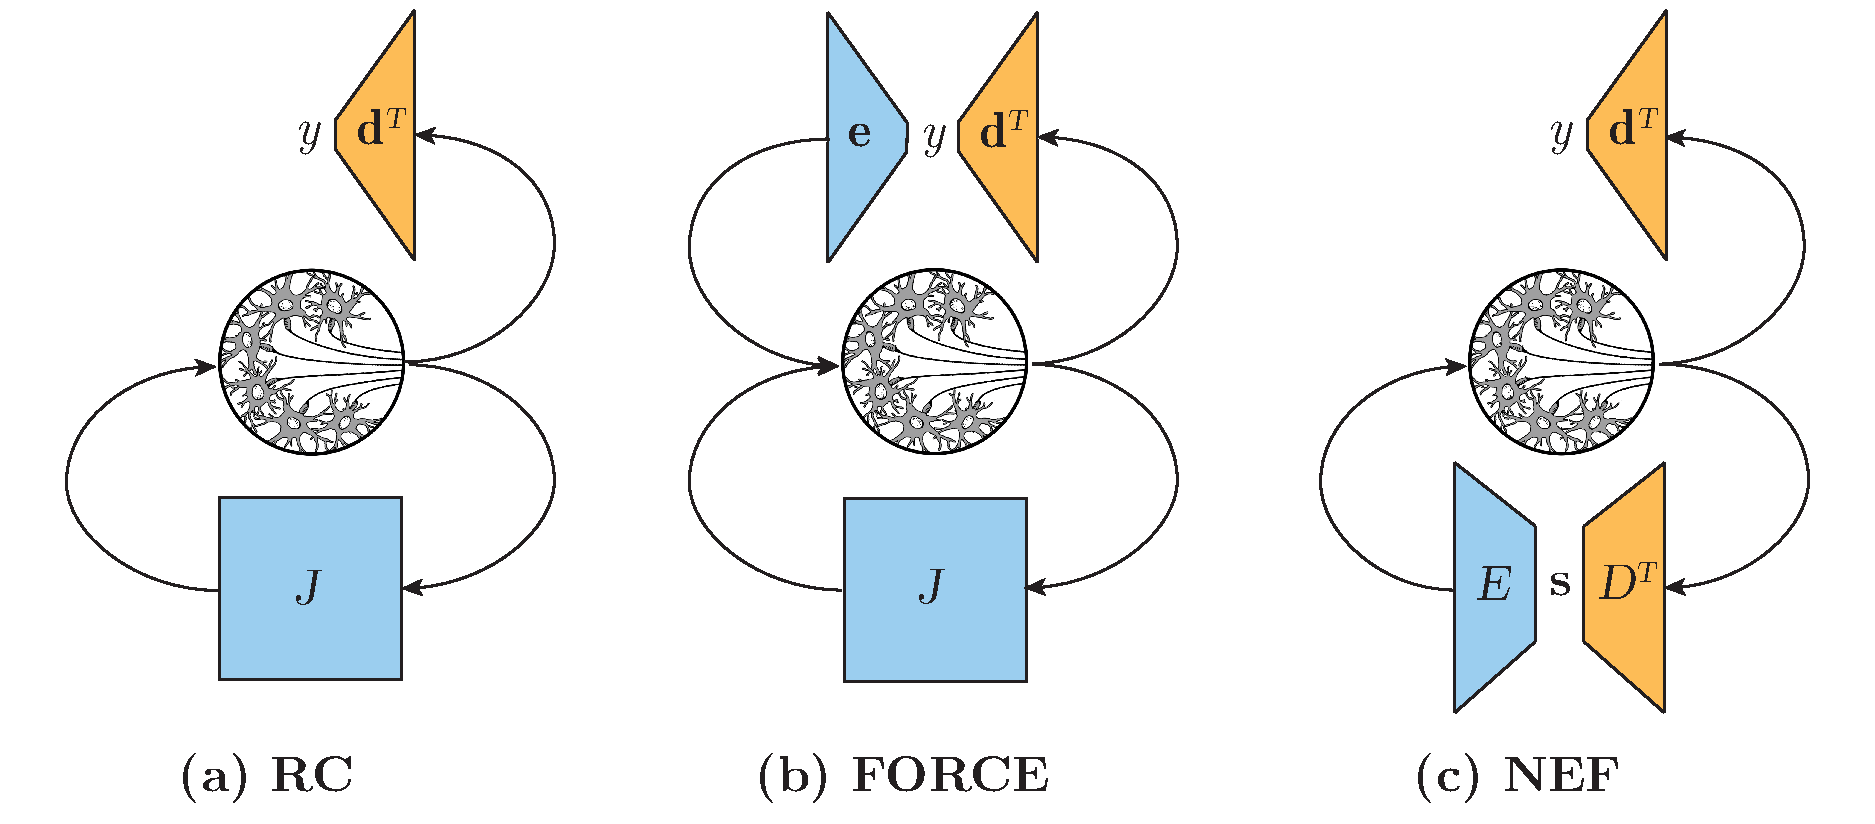
\includegraphics[width=\textwidth]{rc-force-nef.pdf}
  \caption{ \label{fig:architectures}
    Comparing the recurrent architectures of (a)~Reservoir Computing~(RC), (b)~First-Order Reduced and Controlled Error~(FORCE), and (c)~the Neural Engineering Framework~(NEF).
    Blue weights are fixed and randomly chosen.
    Orange weights are learned either online or offline.
    Each ensemble is a pool of synapses and neurons that filter and nonlinearly encode the weighted activities.
    The input to each network is omitted for simplicity.
  }
\end{figure}

To bypass this problem, Reservoir Computing~(RC) has taken a specialized approach to training RNNs (see Figure~\ref{fig:architectures}a).
In essence, RC networks relax the training problem by leaving the recurrent weights fixed.
The two major variants of RC networks are Echo State Networks~\citep[ESNs;][]{jaeger2001echo} and Liquid State Machines~\citep[LSMs;][]{maass2002real}, which differ primarily by their use of rate-based and spiking neurons, respectively.
In either case, RC networks make a conceptual separation between a fixed {\it reservoir} of randomly connected neural units, and a learned {\it readout}.
The reservoir is driven by {\it encoding} the input signal, $u(t) \in \mathbb{R}$ using a random vector, $\V{e}^\text{in} \in \mathbb{R}^n$.
The units within the reservoir are recurrently connected using a random matrix, $J \in \mathbb{R}^{n \times n}$.
And a feed-forward readout vector, $\V{d} \in \mathbb{R}^{n}$, is optimized to {\it decode} some target, $y(t) \in \mathbb{R}$.
%In summary,
%\begin{align} \label{eq:architecture-rc}
%\V{b}(t) &= J \V{a}(t) + \V{e}^\text{in} u(t) \\
%y(t) &= \V{d}^T \V{a}(t) \text{.}
%\end{align}
Intuitively, the reservoir extracts nonlinear temporal features---referred to as {\it echoes}---of the input signal, and the readout combines these dynamical traces to approximate the desired target.
Since the readout is typically a linear combination of the reservoir's activity, a solution may be learned via convex least-squares approximation.
In contrast, the reservoir is untrained with dynamical properties that remain fixed independently of the desired task~\citep{lukovsevicius2012reservoir}.

While RC solves the issue of training RNNs, the problem of efficient scaling remains. 
Indeed, as noted by RC theorists, ``just simply creating a reservoir at random is unsatisfactory'' and ``setting up the reservoir such that a good state expansion emerges is an ill-understood challenge in many respects''~\citep{lukovsevicius2012reservoir}.
Generally, the computational power of RC relies upon having a sufficiently large reservoir representing a high-dimensional superset of the required dynamics, ultimately resulting in an inefficient use of resources for many systems.
This becomes problematic when considering the time and memory required to simulate RC networks, which scales as $\bigoh{ n^2 }$, thus making large-scale simulations of the brain computationally prohibitive.
%We use the example of a delay line to highlight these limitations.

The First-Order Reduced and Controlled Error~\citep[FORCE;][]{sussillo2009generating} method extends ESNs by learning a low-rank component of the recurrent weight matrix, that {\it re-encodes} the desired output back into the network (see Figure~\ref{fig:architectures}b).
Specifically, the recurrent weights have an additional outer-product term, $\V{e} \V{d}^T \in \mathbb{R}^{n \times n}$, where $\V{e} \in \mathbb{R}^n$ is a fixed random vector, and the vector $\V{d} \in \mathbb{R}^n$ are the same decoders from before.
By design, these weights decode the desired output and subsequently encode it back into the reservoir, alongside the random mixing from $J$.
This improves the computational abilities of the network, whenever the dynamical state is a static function of the filtered target signal.
We make this condition mathematically precise in section~\ref{sec:force}.
However, this is not always the case. In general, we show that this choice of re-encoding the output signal is sometimes not only suboptimal, but can hinder performance.
These same observations apply to the state-of-the-art ``full-FORCE'' method~\citep{depasquale2018full}, which learns a full-rank matrix that encodes the same state as in FORCE, but using additional degrees of freedom.

The Neural Engineering Framework~\citep[NEF;][]{eliasmith1999developing,eliasmith2003neural} provides an alternative method for building dynamical neural networks (see Figure~\ref{fig:architectures}c).
Rather than relying on random feedback, or always re-encoding the output (in the case of FORCE), the NEF optimizes the recurrent weights to represent the desired dynamical state.
This can be understood as constructing an RC network with an optimized reservoir, although the approaches were developed independently.
In the NEF, the desired dynamical state, $\V{x}(t) \in \mathbb{R}^q$, is either expressed in closed form as a set of dynamical equations (in continuous-time or discrete-time), or provided via time-series data as is more typical within RC.
Then, the recurrent weight matrix is factored into $ED^T \in \mathbb{R}^{n \times n}$, where $E \in \mathbb{R}^{n \times q}$ is a fixed encoding matrix, $D \in \mathbb{R}^{n \times q}$ is a learned decoding matrix, and $\V{s}(t) \in \mathbb{R}^q$ is the decoded vector that is encoded to represent $\V{x}(t)$.
A central observation made by the NEF is that the optimal $\V{s}(t)$ is determined by: $\V{x}(t)$, the model of postsynaptic current~(PSC), and whether the simulation is analog or digital~\citep{voelker2017b}.
We review this in section~\ref{sec:nef}.
%\begin{equation}\label{eq:boxed}
%\V{s}(t) = \sum_{i=0}^k c_i \V{x}^{(i)}(t) \text{,} \quad \V{s}[t] = \sum_{i=0}^k \bar{c}_i \V{x}^{[i]}[t] \text{,}
%\end{equation}
%where $c_i$ are the transfer function coefficients of the analog synapse model, or $\bar{c}_i$ for the digital synapse model, respectively~\cite[][equations~17,19]{voelker2017b}.
In the same way as FORCE, the NEF may include $\V{d}$ as a column of $D$, and $\V{e}$ as a row of $E$, to re-encode $y(t)$ -- equivalent to asserting that $y(t) \in \V{s}(t)$.
This assumption is made if and only if it is helpful~\citep[i.e.,~to perform integration;][]{singh2004}.
If all relevant state-variables are identified, then the high-dimensional dynamics introduced by $J$ do not help.
The $E$ matrix may also be fine-tuned to better represent $\V{x}(t)$ via back-propagation through time~\citep{rasmussen2018nengodl}.


Within the NEF, the important distinction between ESNs and LSMs is captured simply by the choice of $G_i \left[ \cdot \right]$ (see equation~\ref{eq:encoding}).
In either case, we can identify the neural activity of the reservoir with $a_i^\V{x}(t)$, where $\V{x}(t)$ is some \emph{unknown} (latent) state that depends on both $\V{u}(t)$ and the dynamical properties of the reservoir.
Note that characterizing $\V{x}(t)$ is precisely the problem faced when trying to understand what information RC networks are representing.
Regardless, the linear readout amounts to the following approximate nonlinear function of $\V{x}(t)$:
\begin{equation} \label{eq:rc}
\hat{\V{y}}(t) = \sum_{i=1}^n (a_i^\V{x} \ast h)(t) \V{d}^\V{f}_i \text{.}
\end{equation}
This has the same form as equation~\ref{eq:decoding} from principle~2 of the NEF.
The important difference lies in how the decoders $D^\V{f}$ are trained.
Rather than solving for $D^\V{f}$ using equation~\ref{eq:decoder_solution}, the network is explicitly simulated to obtain the exact temporal basis functions.
In general, the RC training method relies on \emph{explicit} simulation, since $\V{x}(t)$ is unknown. In the NEF the simulation is typically \emph{implicit} within principles~1 and~2 but can also be explicit (see Table \ref{tab:learning-types}).

\begin{table} 
\centering
  \label{tab:learning-types}
  
  \begin{tabular}{@{}lcccccc@{}} \toprule
    & \multicolumn{2}{c}{Recurrence} & \multicolumn{2}{c}{Readout} & \multicolumn{2}{c}{Simulation} \\ 
    \cmidrule(l){2-3} \cmidrule(l){4-5} \cmidrule(l){6-7}
    Method & Online & Offline & Online & Offline & Explicit & Implicit \\ 
    \midrule
    RC & & & & \checkmark & \checkmark & \\
    FORCE & \checkmark & - & \checkmark & - & \checkmark & \\
    full-FORCE & \checkmark & - & - & \checkmark & \checkmark & \\
    NEF & - & \checkmark & - & \checkmark & - & \checkmark \\
    \bottomrule
  \end{tabular}
  \caption{Summary of the characteristics of each training method. Dashes (-) denote less commonly advertised use-cases (see text for details).}
%\begin{tabular}{ |c|c|c| } 
%\hline
%  & Online learning & Offline learning \\ 
%\hline
%Explicit simulation & RC* and NEF & RC and NEF  \\ 
%\hline
%Implicit simulation & NEF & NEF \\ 
%\hline
%\end{tabular} \\
\end{table}

The NEF usually avoids explicit simulation because it is generally more costly (especially as the time-step $dt$ becomes small), which is of practical importance when engineering large-scale networks~\citep[e.g.,][]{eliasmith2012large}.
However, the method does have the benefit of automatically refining the distortion error in the decoding induced by the rate-mode approximation of spiking networks used in equation (\ref{eq:decoder_solution}).
Furthermore, the readout can learn to compensate for other approximation errors and even mischaracterizations of the state-variable.

For the non-adaptive, non-spiking, case the training method adds absolutely no improvement---assuming the representation has been correctly characterized.
Overall, the explicit training method is most suitable for applications where the latent state-variables are not easily characterized---often referred to informally as ``training from data''.
Nevertheless, this perspective is beneficial in conceptualizing the role of the recurrent population as a dynamical reservoir.

From the perspective of RC, the NEF provides a way to solve for the recurrent connection weights by imposing a low-dimensional dynamical state $\V{x}(t)$ on the reservoir.
This can be thought of as building a  \emph{structured} reservoir that is optimized for a restricted subset of functions.
Specifically, we may include a set of temporal basis functions (that incorporate prior knowledge of the desired function) using principle~3, and then apply any training method to this specially constructed reservoir.
The readout may still capture nonlinear relationships between the state and the target, and this readout may still be trained from data.
The NEF provides a way to understand the resulting computations, and to systematically relate the dynamics of the state-variables to the parameters of the computational models.
This allows us to, for instance, understand the network-level effects of including different synapse models.
Furthermore, this reduces the cost of simulation time and memory by a factor of $\bigoh{ n }$ for constant dimensionality, since the number of connection weights for RC scale as $\bigoh{ n^2 }$.

The conclusions from this section are similar to those drawn by \citet[][see supplementary~S1]{nicola2016supervised} in comparing NEF networks to the FORCE method~\citep{sussillo2009generating, abbott2016building}.


\section{Neuromorphic Computing}
\label{sec:neuromorphic}

The term \emph{neuromorphic computing}---also known as neuromorphic engineering---refers broadly to the use of specialized hardware to emulate computational principles of biological nervous systems~\citep{mead1989analog, liu2002analog}.
Here, we focus more specifically on the synthesis of spiking neural networks~(SNNs)---in both analog and digital hardware---for low-power, dynamical, brain-like, computation~\citep{boahen2017neuromorph}.

This chapter provides a brief overview of the landscape, with an emphasis placed on state-of-the-art hardware made available to the Centre for Theoretical Neuroscience, at the University of Waterloo, for academic research, namely: SpiNNaker~\citep{furber2014spinnaker}, Braindrop~\citep{braindrop2019}, and Loihi~\citep{davies2018loihi}.
At the same time, this overlaps with the efforts of many companies, including: Applied Brain Research~(ABR), Femtosense, Intel, IBM, Numenta, Qualcomm, BrainChip, General Vision, HRL Laboratories, Brain Corporation, Knowm, Samsung, and Vicarious FP~\citep{marketreport2018, femtosense} -- although we focus primarily on ABR's marriage of Nengo and the NEF with neuromorphic hardware from Femtosense (i.e.,~Braindrop) and Intel (i.e.,~Loihi).
A non-exhaustive list of other architectures, many of which implement NEF networks, are provided in section~\ref{sec:neuromorphic-others}.

Coming from a purely computational-theoretic perspective, there is nothing special about neuromorphic hardware; alternative hardware architectures cannot move beyond what is already Turing-computable.
There is no logical nor physical reason to believe that neurons and synapses somehow enable new computations that were previously unable to be emulated using available technology.
Instead, neuromorphic architectures aim to implement specific classes of algorithms, realized via massively-parallelized event-driven computations that are sparse in both space and time, using dramatically less power~\citep{tang2017sparse}.

The human brain has been estimated to consume as little as $10$--$20$\,fJ on average per ``synaptic event''~\citep{cassidy2014real, boahen2017neuromorph}, totalling approximately $20$\,W across its {\textasciitilde{}}\numprint{e11}~neurons and {\textasciitilde{}}\numprint{e14}~synapses~\citep{koch2014}.
After $30$ years of work~\citep{cassidy2013design}, the state-of-the-art in neuromorphic computing is on the verge of reaching this level of performance, with Braindrop, Loihi, and TrueNorth~\citep{merolla2014million}, each coming within a factor of \numprint{e1}--\numprint{e3} for roughly equivalent measures of energy per synaptic operation and typical network configurations~\citep{braindrop2019}.
Such potential energy savings are not only tremendous, but a prerequisite to reach the exascale (\numprint{e18}) level of computation achieved by the human brain -- unless one has access to a super-computing cluster powered by a nuclear power plant producing on the order of \numprint{e9}~watts~\citep{furber2012build, neurogrid2014}.
However, such power measurements are not straight-forward to interpret, as there are many other factors such as the cost of scaling, flexibility of the hardware, and open questions surrounding whether the energy per synaptic event is the best metric for evaluating system performance, and how much speed, accuracy, and biological detail is necessary~\citep{eliasmith2013build} -- all of which make fair benchmarking an incredibly challenging problem~\citep{stewart2015closed}.

However, improved power-efficiency often comes at the cost of reduced programmability and narrowed application spaces;
the more you know about the problem that you are trying to solve, the more that can be ``baked in'' to the hardware to save energy and space, while sacrificing flexibility.
This fundamental trade-off between being able to solve fewer problems more efficiently, versus more problems less efficiently, is one that the community as a whole is still trying to navigate.
It appears likely there will be no one-size-fits-all solution, and rather a variety of strategies will be needed to mirror the degrees of architectural specificity observed in the human brain.
Yet, there are many common features between neuromorphic hardware architectures, including: parallelism, memory colocated with computational elements, heterogeneity, sparsity, structured connectivity, minimization of spike traffic and synaptic events, and real-time interfacing.
These features are anticipated to provide robust, scalable, and energy-efficient solutions to the domain of tasks where our brains excel: processing sensory information, language and cognition, and motor behaviours -- all dynamically coupled to the time-scales of our environment.

To fully unlock the potential of such hardware, we require significant advances at the intersection of computer science, computational neuroscience, cognitive modelling, electrical engineering, physics, and mathematics.
This involves discovering new algorithms, developing new frameworks, and training the next generation of programmers to think differently about problems -- but the benefits are far-reaching: real-time computation that can in principle scale up to the perceptual, cognitive, and motor capabilities of the human brain, without requiring the energy production of an entire nuclear power plant.

In chapter~\ref{chapt:nef-extensions} we summarize some of the main challenges surrounding the use of neuromorphic hardware, and demonstrate how the NEF solves many of these problems.
More generally, we provide a theoretical framework and extensions to formally understand the class of computations that neuromorphic hardware enables, given its computational elements and constraints, including resource budget and desired precision.
A novel class of algorithms involving temporal computations are explored and analyzed in detail in chapter~\ref{chapt:delays}.
Applications running on neuromorphic hardware are provided in chapter~\ref{chapt:results}.

\subsection{SpiNNaker}

The SpiNNaker\footnote{SpiNNaker stands for ``Spiking Neural Network Architecture''.} project formally began in 2005 as a collaboration between several universities and industrial partners, housed at the University of Manchester, with the primary goals of simulating large-scale SNNs in real-time, and investigating new architectures which ``lead to fundamentally new and advantageous principles for energy-efficient massively-parallel computing''~\citep{spinnakerproject, furber2014spinnaker}.
Secondary goals include providing a balance between power, cost, and programmability, to make SpiNNaker accessible to a wide range of researchers across neuroscience and cognitive modelling communities.

The basic building block of SpiNNaker is a chip multiprocessor~(CMP) containing 18 ARM968 cores and 128\,MB SDRAM~\citep{painkras2013spinnaker, furber2013overview}.
Each core was prescribed to simulate \numprint{e3} spiking neurons and \numprint{e6} synapses, although Nengo's integration doubled this target by achieving \numprint{2000} neurons per core through the use of factorized weight matrices~\citep{mundy2015}.
Each CMP is fully digital, locally synchronous, clocked at some frequency (e.g.,~$200$\,MHz), and allotted some amount of wall time (e.g.,~$1$\,ms) to complete each time-step.
Thus, both neural and synaptic elements are virtualized (i.e.,~reusing the same shared silicon) by time-multiplexing as many computations as possible within each core given the allotted wall time.
Although the limiting factor in scaling each core is predominantly the amount of available SDRAM split between cores, and the volume of spike traffic transmitted between CMPs.
The architecture scales up to $2^{16}$ CMPs---over \numprint{e9}~neurons and \numprint{e12}~synapses---asynchronously connected to one another through a 2D triangular toroidal mesh.
An instantiation that realizes their initial target of 1\% of the human brain, using \numprint{e6} cores, was finally reached as of 2018.

Studies involving power-usage are surprisingly scarce, but one such study demonstrated that scaling to one quarter of a million neurons required less than $30$\,W of power, in the worst-case~\citep{stromatias2013power}, or on the order of \numprint{e5}--\numprint{e6} times more power than a human brain of the same size.\footnote{
The human brain has \numprint{400000} times as many neurons, and uses $20$\,W of power.}
This is a significant improvement upon high-performance computing~(HPC) architectures, which devour at least \numprint{e8} times more power than a human brain~\citep{furber2012build}. 
However, a more recent study by \citet{van2018performance} concluded much more conservatively that SpiNNaker is still a factor of $\numprint{e7}$--$\numprint{e9}$ away from the efficiency of the mammalian brain.\footnote{
The lower-bound on this estimate comes from a hypothetical extrapolation of their results. Furthermore, the range becomes \numprint{e8}--\numprint{e10} if using the estimate of $10$--$20$\,fJ per synaptic event for the brain.}
In this scenario SpiNNaker was outperformed by NEST running on an HPC cluster, and likewise a smaller-scale implementation of an associative memory on SpiNNaker performed comparably to NEST on an Intel Core i7-4710MQ processor~\citep{stockel2017binary}.
Similarly, \citet{knight2018gpus} found that GPUs improved both the simulation time and energy-to-solution for cortical circuit simulations, compared to SpiNNaker and CPU-based HPC hardware.
On the other hand, \citet{sugiarto2016high} estimated that both SpiNNaker and an FPGA provide a $\numprint{e2}$--$\numprint{e3}$-fold improvement over both CPUs and GPUs, on an image processing task. 
Clearly it matters what one is actually scaling towards.

Nengo has been ported to SpiNNaker~\citep{galluppi2012real, mundy2015} and used to run the full Spaun brain model in real-time~\citep{mundy2016real}.
This goal represented a \numprint{e4}-fold speedup over a conventional X86 CPU implementation~\citep{stewart2014large}.
This implementation required significant work by \citet{mundy2016real} to leverage the flexibility of the SpiNNaker architecture, and so we do not go into detail here.
General support has also been added for both supervised learning~\citep{davies2013} and unsupervised learning~\citep{knight2016} to learn human-scale vocabularies online using Nengo (see section~\ref{sec:learn-spinnaker}).
Meanwhile, Nengo has also been deployed on a prototype autonomous robot equipped with a SpiNNaker board to sense and act in real-time~\citep{galluppi2014}.
PyNN has also been ported over to SpiNNaker, further highlighting the flexibility of the architecture~\citep{rhodes2018spynnaker}.
Several other applications of SpiNNaker are reviewed by \citet{rhodes2018spynnaker}, independently of Nengo.

The next generation of SpiNNaker, dubbed SpiNNaker~2, is currently in development with a prototype chip available for testing~\citep{liu2018memory}.
Although Nengo support may not be available any time soon, the hardware promises to improve upon the speed- and power-efficiency of the first generation by use of improved fabrication processes, advanced per-core power management techniques, and specialized hardware acceleration for the exponential function.
\citet{liu2018memory} deploys a deep neural network on the prototype SpiNNaker~2 test chip, realizing power improvements on the order of \numprint{e2} versus a traditional X86 CPU implementation.

\subsection{Braindrop}

Braindrop~\citep{braindrop2019} is a mixed-signal (i.e.,~both analog and digital) neuromorphic architecture that seeks to realize the energy-efficiency of the human brain, without sacrificing the flexibility required to model large-scale cognitive systems such as Spaun~\citep{eliasmith2012}.
This chip was designed explicitly with the NEF in mind, by way of a novel mapping~\citep{voelker2017iscas, neckar2018optimizing}, accompanied by a number of inventive solutions including: temperature-invariance~\citep{abrams2017, reidpint2019, benjamintemp2019}, H-tree routing~\citep{fokserial2018}, sparse encoding by spatial convolution~\citep{feinstein1988hexagonal, braindrop2019}, and decoding by accumulative spike-thinning~\citep{fokthinning2019}.

This collection of work was the product a 5-year collaboration between Stanford, Yale, and the University of Waterloo, and was made possible in this time frame 
by building on more than a decade of experience building---and years of programming---its predecessor, Neurogrid~\citep{neurogrid2014}. 

Leveraging low-level analog transistor physics to emulate the behaviour of individual neurons and synapses.

Dynamical systems approach \citep{arthur2011silicon}

Multicast tree router \citep{merolla2014multicast}

The NEF has been deployed on Neurogrid primarily to implement control algorithms~\citep{dethier2011brain, choudhary2012silicon, menon2014controlling}.

Requires advanced calibration techniques~\citep{kauderer2017calibrating}.

\subsection{Loihi}

\citep{blouw2018a}

\subsection{Others}
\label{sec:neuromorphic-others}

A number of excellent review articles are made available by \citet{bartolozzi1999neuromorphic}, \citet{indiveri2011neuromorphic}, \citet{cassidy2013design}, \citet{eryilmaz2016neuromorphic}, and \citet{cummings2018}.

Some of the earliest examples include \citep{sivilotti1985novel, boahen1989heteroassociative} and \citep{mead1988silicon}.

Spikey, BrainScaleS 1 and 2, SyNAPSE, Dynapse 1 and 2, TrueNorth~\citep{merolla2014million, fischl2018}, DeepSouth, COLAMN, ODIN, ROLLS, Giacomo and Eliasmith, Tripp, Wang and Tapson, STPU, Neuromemristive random projection networks (Dhireesha Kudithipudi)
\TODO{\url{https://link.springer.com/chapter/10.1007/978-3-642-00641-8_38}}
% A scalable multicore architecture with heterogeneous memory structures for dynamic neuromorphic asynchronous processors (dynaps)
% A 65k-neuron 73-mevents/s 22-pj/event asynchronous micro-pipelined integrate-and-fire array transceiver
% Analog computing in a modern context: A linear algebra accelerator case study
% A wafer-scale neuromorphic hardware system for large-scale neural modeling
% A digital neurosynaptic core using embedded crossbar memory with 45 pJ per spike in 45 nm, (GoldenGate SyNAPSE IBM)
\TODO{Cite any ASIC results for deep learning?}

\section{Dynamical Systems}

\subsection{Linear Time-Invariant Systems}

State-space representations, transfer functions, filters, convolution, properties, Pad\'e approximants and coordinate transformations

\subsection{Nonlinear Systems}

Linearization, Jacobians, signatures of chaos

\subsubsection{Coordinate Transformation}

\begin{theorem}
Let $\V{f}(t)$ and $\V{g}(t)$ be infinitely time-differentiable signals, that are related by:
\begin{equation} \label{eq:f}
\V{f} = \sum_{i=0}^\infty c_i \V{g}^{(i)} \text{,}
\end{equation}
for some coordinates $\coords{c}{i}$. Then this dynamical system is equivalent to:
\begin{equation} \label{eq:g}
\V{g} = \sum_{i=0}^\infty b_i \V{f}^{(i)} \text{,}
\end{equation}
where the coordinates $\coords{b}{i}$ are defined by the recursive transformation:
\begin{equation} \label{eq:b}
b_i = c_0^{-1} \begin{cases}
    1 & i = 0 \\
    %- (b \ast c)\left[ i \right] & i \ge 1 ,
    - \sum_{j=0}^{i-1} b_j c_{i - j} & i \ge 1 \text{.}
  \end{cases}
\end{equation}
%and $(b \ast c)\left[ i \right] := \sum_{j=0}^{i-1} b_j c_{i - j}$ is a discrete convolution. % that depends on $b_j$ for all $0 \le j \le i - 1$.
\end{theorem}

\begin{corollary}
Let: $$H_c(s) = \frac{1}{\sum_{i=0}^\infty c_i s^i}, \quad H_b(s) = \frac{1}{\sum_{i=0}^\infty b_i s^i}, $$ where $b$ is defined by (\ref{eq:b}). Then (\ref{eq:f}) is equivalent to $F(s)H_c(s) = G(s)$ and similarly (\ref{eq:g}) is equivalent to $G(s)H_b(s) = F(s)$, and moreover:
\begin{equation} \label{eq:inv}
H_c(s) H_b(s) = 1 \text{,}
\end{equation}
hence $H_c(s)$ and $H_b(s)$ are eachother's reciprocals. Furthermore, the coordinate transformation (\ref{eq:b}) is its own inverse.
\end{corollary}

\begin{proof}
Noting that $\V{g}^{(0)} = \V{g}$, rearrange (\ref{eq:f}) as:
\begin{equation} \label{eq:gf}
\V{g} = c_0^{-1} \V{f} + \sum_{i=1}^\infty (-c_0^{-1} c_i) \V{g}^{(i)} \text{.}
\end{equation}
Differentiate each side an infinite number of times, to obtain the following set of equations that hold for all $j \in \mathbb{N}$:
\begin{equation} \label{eq:dg}
\V{g}^{(j)} = c_0^{-1} \V{f}^{(j)} + \sum_{i=1}^\infty (-c_0^{-1} c_i) \V{g}^{(i+j)} \text{.}
\end{equation}
Now recursively substitute (\ref{eq:dg}) into (\ref{eq:gf}) for all occurrences of $\V{g}^{(i)}$, $i \ge 1$ until we are only left with $\V{f}^{(j)}$ terms for $j \le i$, and take the limit as $i \rightarrow \infty$. This is equivalent to treating (\ref{eq:dg}) as a recursive function in $j$ and then evaluating $\V{g}^{(0)}$.
Although this is infinitely generative from a bottom-up perspective, we are `allowed' to do this because each substitution of (\ref{eq:dg}) increases the order of $\V{g}$ by 1 (hence it terminates top-down). Another way to view this is we pick some finite $k$ in order to gather all occurrences of $\V{f}^{(k)}$ in the infinite expansion. After repeating this for all $k \rightarrow \infty$, we get something of the form:
\begin{equation*}
\V{g} = \sum_{k=0}^\infty \tilde{b}_k \V{f}^{(k)} \text{.}
\end{equation*}
Now, all that remains is to show that $\tilde{b}_k = b_k$ from (\ref{eq:b}) in order to match (\ref{eq:g}). We do this inductively in a way that parallels the recursive structure of the substitution procedure.

For the base case ($k = 0$) it should be clear that $\tilde{b}_0 = c_0^{-1} = b_0$ since this is the only way to construct $\V{f}^{(0)}$.
For the inductive case ($k \ge 1$), the only way to construct $\V{f}^{(k)}$ is through the substitution of $\V{g}^{(k)}$ in (\ref{eq:dg}).
Furthermore, this occurs for all $0 \le j \le k - 1$. In particular, for every such $j$, we have the coefficient $(-c_0^{-1} c_{i})$ multiplied by $\V{g}^{(i + j)}$ to yield $c_0^{-1} \V{f}^{(k)}$ where $k = i + j$.
Finally, this occurs $\tilde{b}_{j} c_0$ times since it is mirrored by each occurrence of $\V{f}^{(j)}$.
Putting this all together, we get $\tilde{b}_k = \sum_{j=0}^{k-1} -c_0^{-1} c_{k - j} \tilde{b}_j = c_0^{-1} \sum_{j=0}^{k-1} - b_j c_{k - j} = b_k$ (by the inductive hypothesis).
\end{proof}

\TODO{Move Example later on when citing ISCAS paper}

This theorem is a more general version of the analysis we do in ISCAS~2017. To be concrete, we have:
$$
\V{f} = (\epsilon \gamma)^{-1} \left( \V{x} + (\tau_1 + \tau_2) \dot{\V{x}} + \tau_1 \tau_2 \ddot{\V{x}} \right) \text{,}
$$
$$
c_i = \frac{(-\epsilon)^i}{(i + 1)!} \text{,}
$$
and $\V{g}$ is the signal being used to drive the pulse-extender, such that $\V{f} = \sum_{i=0}^\infty c_i \V{g}^{(i)}$ (see my other notes on improving Kwabena's box filter analysis).

In my refined analysis, we only keep the terms $i \le 2$ (or $i \le 1$ in the paper), but we can still use the above coordinate transformation as a sanity check. In particular, we have:
$$
c_0 = 1, \quad c_1 = -\frac{\epsilon}{2}, \quad c_2 = \frac{\epsilon^2}{6}, \quad c_3 = -\frac{\epsilon^3}{24}, \quad c_i \approx 0 \quad \forall i \ge 4 \text{.}
$$
Then using the transformation (\ref{eq:b}), we get:
$$
b_0 = 1, \quad b_1 = \frac{\epsilon}{2}, \quad b_2 = \frac{\epsilon^2}{4} - \frac{\epsilon^2}{6} = \frac{\epsilon^2}{12}, \quad b_3 = \frac{\epsilon^3}{24} - \frac{\epsilon^3}{12} + \frac{\epsilon^3}{24} = 0 \text{,}
$$
and so:
\begin{align*}
\V{g} &= \sum_{i=0}^\infty b_i \V{f}^{(i)} \\
        &= \V{f}^{(0)} + \frac{\epsilon}{2} \V{f}^{(1)} + \frac{\epsilon^2}{12} \V{f}^{(2)} + \ldots \\
        &= (\epsilon \gamma)^{-1} \left( \V{x} + (\tau_1 + \tau_2 + \epsilon / 2) \dot{\V{x}} + (\tau_1 \tau_2 + (\epsilon / 2 ) (\tau_1 + \tau_2) + \epsilon^2 / 12) \ddot{\V{x}} \right) + \ldots
\end{align*}

The coordinate transformation (\ref{eq:b}) is equivalent to finding the Pad\'e approximants when the order of the numerator is $p = 0$.
To be precise,
$$
\sum_{i=0}^{q} c_i x^i \approx \frac{1}{\sum_{i=0}^q b_i x^i}
$$
is best-approximated by taking the Pad\'e approximants:
$$
\coords{b}{i=0 \ldots q} = \left[ 0 / q \right] \sum_{i=0}^{q} c_i x^i \text{.}
$$
This can be seen through (\ref{eq:inv}) and verified by comparing the algorithm for the extended euclidean algorithm for the polynomial GCD, in this special case, to the algorithm (\ref{eq:b}). That is, they both implement long division.

Despite the fact that we essentially re-derived a special case of the Pad\'e approximants, this still leads to some non-trivial insights:

The coordinate transformation (\ref{eq:b})---that is, the algorithm for finding the Pad\'e approximants when $p = 0$---is its own inverse. That is, we may convert back and forth using the same transformation without any loss of information.

We may also interpret (\ref{eq:b}) as a discrete dynamical system by realizing that $b$ is the discrete convolution of itself with $c$. With some work, we can show that this is the same as stating that $\ztrans{b}\ztrans{c} = 1$, or equivalently in the time-domain, $\coords{b}{i=0\ldots q}$ is the impulse-response of the following discrete transfer function:
$$
H^q_{c \rightarrow b}(z) = \frac{z^{q}}{\sum_{i=0}^q c_i z^{q - i}} \text{,}
$$
and likewise, $H^q_{b \rightarrow c}(z)$ has the impulse-response $\coords{c}{i=0\ldots q}$.
Furthermore, $$\lim_{q \rightarrow \infty} H^q_{c \rightarrow b}(z) H^q_{b \rightarrow c}(z) = 1,$$ analogous to (\ref{eq:inv}).
